% * Week 3. (Aug 10) Regression for prediction. Ch3 (Rob)
%   - Lecture 5: Review of linear regression, matrix formulation
%   - Lab 3:
%   - Lecture 6: Subset selection, LOOCV 


\documentclass[14pt]{beamer}
\usepackage{pgf,tikz,pgfpages,amsmath,bm,fancyvrb,animate}
\usepackage{graphicx,bera,booktabs}
\usepackage[australian]{babel}
\usepackage[utf8]{inputenc}

\usetheme{Monash}
\def\biz{\begin{itemize}[<+-| alert@+>]}
\def\eiz{\end{itemize}}
\def\ben{\begin{enumerate}[<+-| alert@+>]}
\def\een{\end{enumerate}}

\graphicspath{{figs/}}

\title[2. Statistical learning]{Business Analytics}
\author{2. Statistical learning}


\DefineShortVerb{\"}
\def\FancyVerbFormatCom{\color[rgb]{0.6,0,1}\relax}


\begin{document}

\begin{frame}[plain]{}
\maketitle
\begin{textblock}{11}(0.5,1.19){\color{white}\large
\textbf{ETC3250}}
\end{textblock}
\end{frame}

\section{Revision: multiple regression}


\begin{frame}{Revision: Multiple regression}

\begin{block}{}\vspace*{-0.75cm}
$$Y_i = \beta_0 + \beta_1 X_{1,i} + \beta_2 X_{2,i} + \cdots + \beta_kX_{k,i} + e_i.$$
\end{block}
\biz
\item Each $X_{j,i}$ is numerical and is called a ``predictor''.

\item The coefficients $\beta_1,\dots,\beta_k$ measure the effect of each
predictor after taking account of the effect of all other predictors
in the model.

\item That is, the coefficients measure the \textbf{marginal effects}.

\eiz

\end{frame}




\begin{frame}{Credit scores}

Banks score loan customers based on a lot of personal information. A sample of 500 customers from an Australian bank provided the following information.

\hspace*{-0.3cm}{\footnotesize
\begin{tabular}{rrrrr}
  \hline
\bf Score & \bf Savings & \bf Income & \bf Time current address & \bf Time current job \\
& \$'000 & \$'000 & Months & Months \\
  \hline
39.40 & 0.01 & 111.17 &  27 &   8 \\
  51.79 & 0.65 & 56.40 &  29 &  33 \\
  32.82 & 0.75 & 36.74 &   2 &  16 \\
  57.31 & 0.62 & 55.99 &  14 &   7 \\
  37.17 & 4.13 & 62.04 &   2 &  14 \\
  33.69 & 0.00 & 43.75 &   7 &   7 \\
  25.56 & 0.94 & 79.01 &   4 &  11 \\
  32.04 & 0.00 & 45.41 &   3 &   3 \\
  41.34 & 4.26 & 55.22 &  16 &  18 \\
  \vdots & \vdots & \vdots & \vdots & \vdots\\
%  26.72 & 0.01 & 55.03 &  10 &  32 \\
%   \hline
\end{tabular}
}

\only<2>{\begin{textblock}{9}(3,5)
\begin{block}{}Can we use only savings, income, time @ address and time employed to predict the score of a new customer?\end{block}
\end{textblock}}

\end{frame}

\begin{frame}{Credit scores}
\only<1>{\placefig{4.4}{1.4}{height=8.6cm,trim=20 0 0 25,clip=TRUE}{scores1}}
\only<2>{\placefig{4.4}{1.4}{height=8.6cm,trim=20 0 0 25,clip=TRUE}{scores2}
\begin{textblock}{4}(0,1.5)\small
\biz
\item Taking logarithms reduces the skewness in the predictor variables.
\item Because of zeros, I used $\log(x+1)$.
\eiz
\end{textblock}}
\end{frame}

\begin{frame}{Credit scores}

\structure{Proposed model}
\begin{block}{}
\centerline{$ Y = \beta_0 + \beta_1X_1 + \beta_2X_2 + \beta_3X_3 + \beta_4X_4 + e$}
\end{block}
\begin{align*}
\text{where~~}
Y     &=  \text{Credit score},         \\
X_{1} &=  \text{log savings}, \\
X_{2} &=  \text{log income},      \\
X_{3} &=  \text{log time at current address},\\
X_4     &=  \text{log time in current job},\\
e     &=  \text{error}.
\end{align*}



\end{frame}


\begin{frame}[fragile]{Credit scores}\footnotesize

\structure{Computer output from fitting model}

\begin{verbatim}
Coefficients:
             Estimate Std. Error t value Pr(>|t|)
(Intercept)    -0.219      5.231   -0.04   0.9667
log.savings    10.353      0.612   16.90  < 2e-16
log.income      5.052      1.258    4.02  6.8e-05
log.address     2.667      0.434    6.14  1.7e-09
log.employed    1.314      0.409    3.21   0.0014

Residual standard error: 10.2 on 495 degrees of freedom
Multiple R-squared: 0.47,       Adjusted R-squared: 0.466
F-statistic:  110 on 4 and 495 DF,  p-value: <2e-16
\end{verbatim}
\end{frame}

\begin{frame}{Credit scores}
\fullheight{scores3}
\only<2->{\begin{textblock}{3}(2,2){\color{red}
Correlation:\vspace*{-0.5cm} \begin{align*}r &= 0.6856\\
r^2 &= 0.4701\end{align*}}\end{textblock}}
\only<3->{\begin{textblock}{5.5}(7,6.7){\color{blue}\footnotesize
About half the variation in scores can be predicted using this model.}
\end{textblock}}
\end{frame}


\begin{frame}{Credit scores}\vspace*{-0.2cm}
\structure{Residual (or error)}

\begin{tabular}{lccl}
$e_i =$ & $Y_i$ & \hspace*{-0.8cm}$-$ & $\hat Y_i$ \\
& $\uparrow$ & & $\uparrow$ \\
& \hspace*{-0.8cm}(observed) & & \hspace*{-0.4cm}(estimated using regression model)
\end{tabular}

\pause

\centerline{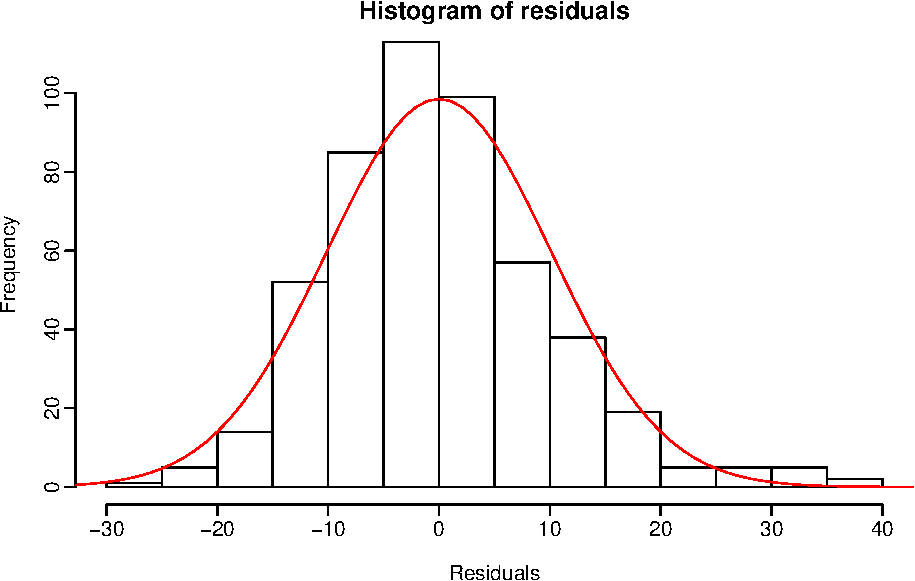
\includegraphics[height=6cm]{scores6}}

\end{frame}

\begin{frame}{Credit scores}
\only<1>{\fullheight{scores4}}
\only<2>{\fullheight{scores5}}
\end{frame}


\begin{frame}{Residual plots}

Useful for spotting outliers and whether the straight line was
appropriate.

\biz
\item Scatterplot of residuals $e_i$ against the predictor
$X_i$.

\item Scatterplot residuals against the fitted values $\hat Y_i$

\item Expect to see scatterplots resembling a horizontal band with
no values too far from the band and no patterns such as curvature or
increasing spread.
\eiz

\end{frame}

\begin{frame}{Residual plots}\small\vspace*{-0.4cm}

\centerline{\includegraphics[width=8cm]{pulpres}}

{Residual plot from the Pulp regression.  Here the residuals show a
V-shaped pattern. This indicates the straight line relationship was
not appropriate for these \rlap{data.}}

\end{frame}






\section{Matrix formulation}

\begin{frame}{Matrix formulation}

\begin{block}{}\vspace*{-0.75cm}
$$Y_i = \beta_0 + \beta_1 X_{1,i} + \beta_2 X_{2,i} + \cdots + \beta_kX_{k,i} + e_i.$$
\end{block}\pause

Let $\bm{Y} = (Y_1,\dots,Y_n)'$, $\bm{e} = (e_1,\dots,e_n)'$, $\bm{\beta} = (\beta_1,\dots,\beta_k)'$ and
\[
\bm{X} = \begin{bmatrix}
  1 & X_{1,1} & X_{2,1} & \dots & X_{k,1}\\
  1 & X_{1,2} & X_{2,2} & \dots & X_{k,2}\\
\vdots & \vdots & \vdots & & \vdots\\
  1 & X_{1,n} & X_{2,n} & \dots & X_{k,n}
  \end{bmatrix}.
\]\pause

Then
\begin{block}{}\vspace*{-0.35cm}
$$\bm{Y} = \bm{X}\bm{\beta} + \bm{e}.$$
\end{block}
\end{frame}

\begin{frame}{Matrix formulation}

\structure{Least squares estimation}

Minimize: $(\bm{Y} - \bm{X}\bm{\beta})'(\bm{Y} - \bm{X}\bm{\beta})$\pause
\vspace*{0.5cm}

Differentiate wrt $\bm{\beta}$ gives

\begin{block}{}\vspace*{-0.2cm}
\[
\hat{\bm{\beta}} = (\bm{X}'\bm{X})^{-1}\bm{X}'\bm{Y}
\]
\end{block}
\pause
(The ``normal equation''.)\pause

\[
\hat{\sigma}^2 = \frac{1}{n-k-1}(\bm{Y} - \bm{X}\hat{\bm{\beta}})'(\bm{Y} - \bm{X}\hat{\bm{\beta}})
\]
\vspace*{.2cm}

\structure{Note:} If you fall for the dummy variable trap, $(\bm{X}'\bm{X})$ is a singular matrix.
\end{frame}


\begin{frame}{Likelihood}

If the errors are iid and normally distributed, then
\[
\bm{Y} \sim \text{N}(\bm{X}\bm{\beta},\sigma^2\bm{I}).
\]\pause
So the likelihood is
\[
L = \frac{1}{\sigma^n(2\pi)^{n/2}}\exp\left(-\frac1{2\sigma^2}(\bm{Y}-\bm{X}\bm{\beta})'(\bm{Y}-\bm{X}\bm{\beta})\right)
\]\pause
which is maximized when $(\bm{Y}-\bm{X}\bm{\beta})'(\bm{Y}-\bm{X}\bm{\beta})$ is minimized.\pause

\centerline{\textcolor[rgb]{0.80,0.00,0.00}{So \textbf{MLE = OLS}.}}
\end{frame}


\begin{frame}{Multivariate statistics}

Let $\bm{Y}$ be a random vector with mean $\bm{\mu}$ and covariance matrix $\bm{V}$.

Let $\bm{A}$ and $\bm{B}$ be constant matrices.

\pause

\begin{block}{Moments of linear functions}
\biz
\item $\E(\bm{A}+\bm{B}\bm{Y}) = \bm{A}+\bm{B}\bm{\mu}$
\item $\V(\bm{A}+\bm{B}\bm{Y}) = \bm{B}\bm{V}\bm{B}'$
\eiz
\end{block}

\end{frame}

\begin{frame}{Multiple regression forecasts}

\begin{block}{Optimal forecasts}\vspace*{-0.7cm}
\[
\hat{Y}^* =
\text{E}(Y^* | \bm{Y},\bm{X},\bm{X}^*) =
\bm{X}^*\hat{\bm{\beta}} = \bm{X}^*(\bm{X}'\bm{X})^{-1}\bm{X}'\bm{Y}
\]
\end{block}
where $\bm{X}^*$ is a row vector containing the values of the regressors for the forecasts (in the same format as $\bm{X}$).\vspace*{0.cm}

\pause

\begin{block}{Forecast variance}\vspace*{-0.7cm}
\[
\text{Var}(Y^* | \bm{Y},\bm{X},\bm{X}^*) = \sigma^2 \left[1 + \bm{X}^* (\bm{X}'\bm{X})^{-1} (\bm{X}^*)'\right]
\]
\end{block}\pause

\biz
\item This ignores any errors in $\bm{X}^*$.

\item 95\% prediction intervals assuming normal errors:
$  \hat{Y}^* \pm 1.96 \sqrt{\text{Var}(Y^*| \bm{Y},\bm{X},\bm{X}^*)}
$.
\eiz

\end{frame}

\begin{frame}{Multiple regression forecasts}


\begin{block}{Fitted values}\vspace*{-0.7cm}
\[
\hat{\bm{Y}} =
\text{E}(\bm{Y}|\bm{X}) =
\bm{X}\hat{\bm{\beta}} = \bm{X}(\bm{X}'\bm{X})^{-1}\bm{X}'\bm{Y} = \bm{H}\bm{Y}
\]
\end{block}
where $\bm{H} = \bm{X}(\bm{X}'\bm{X})^{-1}\bm{X}'$ is the ``hat matrix''.\pause

\structure{Leave-one-out residuals}

Let $h_1,\dots,h_n$ be the diagonal values of $\bm{H}$, then the cross-validation statistic is
\begin{block}{}
\centerline{$\displaystyle
\text{CV} = \frac1n\sum_{i=1}^n[e_i/(1-h_i)]^2,$}
\end{block}
where $e_i$ is the residual obtained from fitting the model to all $n$ observations.


\end{frame}



\section{Choosing regression variables}

\begin{frame}{Choosing regression models}
\biz
\item When there are many predictors, how should we choose which ones to use?

\item We need a way of comparing two competing models

\item If there are a limited number of predictors, we can study all possible models.

\item Otherwise we need a search strategy to explore some potential models.
\eiz

\end{frame}


\begin{frame}{Choosing regression variables}


\structure{What not to do!}
\biz
\item Plot $Y$ against a particular predictor ($X_j$)
       and if it shows no noticeable relationship,  drop it.

%\item Look  at  correlations among the predictors
%       (all of the potential candidates)  and every time a large
%       correlation is encountered,  remove one of  the  two
%       variables from further consideration.

\item Do a multiple linear regression on all the predictors
      and
      disregard all variables whose  $p$ values are greater than 0.05.

\item Maximize $R^2$

\item Minimize SSE.
\eiz
\end{frame}%

\begin{frame}{Comparing regression models}
\structure{Sum of squared errors}
\[\text{SSE} = \sum_{i=1}^n e_i^2 \]
Minimizing SSE will always choose the model with the most predictors.

\pause
\structure{Estimated residual variance}
\[
\hat{\sigma}^2 = \frac{\text{SSE}}{n-k-1}
\]
where $k=$ no.\ predictors.\pause

Minimizing $\hat{\sigma}^2$ works quite well for choosing predictors (but better methods to follow).

\end{frame}
\begin{frame}{Comparing regression models}

Computer output for regression will always give the $R^2$ value. This is a
useful summary of the model.
\biz%\parskip=2ex
\item It is equal to the square of the correlation between $Y$ and $\hat Y$.

\item It is often called the ``coefficient of determination''.

\item It can also be calculated as follows:
$$R^2 = \frac{\sum(\hat{Y}_i - \bar{Y})^2}{\sum(Y_i-\bar{Y})^2}
$$

\item It is
the proportion of variance accounted for (explained) by the predictors.
\eiz
\end{frame}

\begin{frame}{Comparing regression models}

However \dots
\biz
\item $R^2$  does not allow for ``degrees of \rlap{freedom''.}

\item Adding \textit{any} variable tends to increase the value of $R^2$, even if that variable is
\rlap{irrelevant.}
\eiz\pause

To overcome   this problem, we can use \rlap{\emph{adjusted $R^2$}:}
\begin{block}{}
\[
\bar{R}^2 = 1-(1-R^2)\frac{n-1}{n-k-1}
\]
\end{block}
\pause

\centerline{\textcolor[rgb]{0.8,0.00,0.00}{\textbf{Maximizing $\bar{R}^2$ is equivalent to minimizing $\hat\sigma^2$.}}}

%$\bar{R}^2$    is  referred  to  as
%``adjusted $R^2$'' or ``$R$-bar-squared,''    or sometimes as  ``$R^2$,
%corrected for degrees of freedom.''
\end{frame}


\begin{frame}{Cross-validation}

Leave-one-out cross-validation for regression can be carried out using the following steps.
\ben
\item Remove observation $i$ from the data set, and fit the model using the remaining data. Then compute the error ($e_i^*=y_i-\hat{y}_i$) for the omitted observation.
\item Repeat step 1 for $i=1,\dots,n$.
\item Compute the MSE from $\{e_1^*,\dots,e_n^*\}$. We shall call this the CV.
\een\pause
The best model is the one with the smallest value of CV.
\end{frame}

\begin{frame}{Akaike's Information Criterion}

\begin{block}{}
\[
\text{AIC} = -2\log(L) + 2(k+1)
\]
\end{block}
where $L$ is the likelihood and $k$ is the number of predictors in the model.\pause

\biz
\item This is a \emph{penalized likelihood} approach.

\item \emph{Minimizing} the AIC gives the best model for prediction.

\item AIC penalizes terms more heavily than $\bar{R}^2$.

\item Minimizing the AIC is asymptotically equivalent to minimizing MSE via leave-one-out cross-validation.
\eiz

\end{frame}

\begin{frame}{Corrected AIC}

For small values of $n$, the AIC tends to select too many predictors, and so a bias-corrected version of the AIC has been developed.
\begin{block}{}
\[
\text{AIC}_{\text{C}} = \text{AIC} + \frac{2(k+2)(k+3)}{n-k-1}
\]
\end{block}
As with the AIC, the AIC$_{\text{C}}$ should be minimized.
\end{frame}

\begin{frame}{Schwartz Bayesian Information Criterion}

\begin{block}{}
\[
\text{BIC} = -2\log(L) + (k+1)\log(n)
\]
\end{block}
where $L$ is the likelihood and $k$ is the number of predictors in the model.\pause

\biz
\item \emph{Minimizing} the BIC gives the best model for prediction.

\item BIC penalizes terms more heavily than \rlap{AIC}

\item Also called SBIC and SC.

\item Minimizing BIC is asymptotically equivalent to leave-$v$-out cross-validation when $v = n[1-1/(log(n)-1)]$.

\eiz

\end{frame}


\begin{frame}{Choosing regression variables}

\structure{Best subsets regression}

\biz
\item
Fit all possible regression models using one or more of the predictors.

\item
Choose the best model based on one of the measures of predictive ability (CV, AIC, AICc, BIC, $\bar{R}^2$).
\eiz

\vfill\pause

\structure{Warning!}
\begin{itemize}
\item If there are a large number of predictors, this is not possible.

For example, 44 predictors leads to 18 trillion possible models!
\end{itemize}

\end{frame}



\begin{frame}{Choosing regression variables}\footnotesize\vspace*{-0.2cm}
{\tabcolsep=0.1cm
\hspace*{-0.7cm}\begin{tabular}{ccccccccc}
  \hline
 Savings & Income & Address & Employed & CV & AIC & AICc & BIC & $\bar{R}^2$ \\
  \hline
  X & X & X & X & 104.7 & 2325.8 & 2325.9 & 2351.1 & 0.4658 \\
  X & X & X &   & 106.5 & 2334.1 & 2334.2 & 2355.1 & 0.4558 \\
  X &   & X & X & 107.7 & 2339.8 & 2339.9 & 2360.9 & 0.4495 \\
  X &   & X &   & 109.7 & 2349.3 & 2349.3 & 2366.1 & 0.4379 \\
  X & X &   & X & 112.2 & 2360.4 & 2360.6 & 2381.5 & 0.4263 \\
  X &   &   & X & 115.1 & 2373.4 & 2373.5 & 2390.3 & 0.4101 \\
  X & X &   &   & 116.1 & 2377.7 & 2377.8 & 2394.6 & 0.4050 \\
  X &   &   &   & 119.5 & 2392.1 & 2392.2 & 2404.8 & 0.3864 \\
    & X & X & X & 164.2 & 2551.6 & 2551.7 & 2572.7 & 0.1592 \\
    & X & X &   & 164.9 & 2553.8 & 2553.9 & 2570.7 & 0.1538 \\
    & X &   & X & 176.1 & 2586.7 & 2586.8 & 2603.6 & 0.0963 \\
    &   & X & X & 177.5 & 2591.4 & 2591.5 & 2608.3 & 0.0877 \\
    &   & X &   & 178.6 & 2594.6 & 2594.6 & 2607.2 & 0.0801 \\
    & X &   &   & 179.1 & 2595.3 & 2595.3 & 2607.9 & 0.0788 \\
    &   &   & X & 190.0 & 2625.3 & 2625.4 & 2638.0 & 0.0217 \\
    &   &   &   & 193.8 & 2635.3 & 2635.3 & 2643.7 & 0.0000 \\
   \hline
\end{tabular}}

\end{frame}


\begin{frame}{What to use?}

\structure{Choice: BIC, CV, AICc, AIC, $\bar{R}^2$.}
\pause
\biz
\item BIC tends to choose models too small for prediction.

\item As $n\rightarrow\infty$, BIC selects \emph{true} model if there is one.

\item $\bar{R}^2$ tends to select models too large.

\item AIC also slightly biased towards larger models (but only when $n$ is small).

\item Empirical studies in forecasting show AIC is better than BIC for forecast accuracy.
\eiz
\end{frame}

\begin{frame}[squeeze,shrink=0.99]{Choosing regression variables}
\structure{Backwards stepwise regression}

\biz
\item Start with a model containing all variables.

\item Try subtracting one variable at a time. Keep the model if it
has lower \rlap{CV, AICc or AIC.}

\item Iterate until no further improvement.
\eiz

\pause%\small

\structure{\textcolor[rgb]{0.80,0.00,0.00}{Notes:}}
\biz\itemsep=0cm\parskip=0cm
%\item Putting all the predictors in can lead to a significant
%\textit{overall effect} but with no way of determining the individual effects
%of each variable.
%
%\item Using stepwise regression is useful for choosing only the most
%significant variables in the regression model.

\item Stepwise regression is not guaranteed to lead to the best possible
model.

\item If you are trying several different models, use the CV, AICc or AIC %adjusted $R^2$
value to select between them.
\eiz

\end{frame}

\begin{frame}[fragile]{R example}\footnotesize
\begin{verbatim}
lm(formula = score ~ log.savings, data = creditlog)

Coefficients:
            Estimate Std. Error t value Pr(>|t|)    
(Intercept)  29.3227     0.6448   45.48   <2e-16 ***
log.savings  11.2702     0.6348   17.75   <2e-16 ***
---
Signif. codes:  0 '***' 0.001 '**' 0.01 '*' 0.05 '.' 0.1 ' ' 1 

Residual standard error: 10.89 on 498 degrees of freedom
Multiple R-squared: 0.3876, Adjusted R-squared: 0.3864 
F-statistic: 315.2 on 1 and 498 DF,  p-value: < 2.2e-16 

   CV  AIC AICc  BIC   AdjR2
119.5 2392 2392 2405 0.38639
\end{verbatim}
\vspace*{10cm}

\end{frame}

\begin{frame}[fragile]{R example}\footnotesize
\begin{verbatim}
lm(formula = score ~ log.savings + log.employed, data = creditlog)

Coefficients:
             Estimate Std. Error t value Pr(>|t|)
(Intercept)    24.343      1.257   19.37  < 2e-16
log.savings    11.287      0.622   18.13  < 2e-16
log.employed    1.927      0.420    4.58  5.8e-06

Residual standard error: 10.7 on 497 degrees of freedom
Multiple R-squared: 0.412,  Adjusted R-squared: 0.41 
F-statistic:  174 on 2 and 497 DF,  p-value: <2e-16 

   CV  AIC AICc  BIC   AdjR2
115.1 2373 2373 2390 0.41010
\end{verbatim}
\vspace*{10cm}

\end{frame}

\begin{frame}[fragile]{R example}\footnotesize
\begin{verbatim}
lm(formula = score ~ log.savings + log.address + log.employed, 
    data = creditlog)

Coefficients:
             Estimate Std. Error t value Pr(>|t|)
(Intercept)    20.039      1.407   14.24  < 2e-16
log.savings    10.934      0.604   18.10  < 2e-16
log.address     2.668      0.441    6.05  2.9e-09
log.employed    1.406      0.415    3.39  0.00076

Residual standard error: 10.3 on 496 degrees of freedom
Multiple R-squared: 0.453,  Adjusted R-squared: 0.45 
F-statistic:  137 on 3 and 496 DF,  p-value: <2e-16 

   CV  AIC AICc  BIC   AdjR2
107.7 2340 2340 2361 0.44952
\end{verbatim}
\vspace*{10cm}

\end{frame}

\begin{frame}[fragile]{R example}\footnotesize
\begin{verbatim}
lm(formula = score ~ log.savings + log.income + log.address + 
    log.employed, data = creditlog)

Coefficients:
             Estimate Std. Error t value Pr(>|t|)
(Intercept)    -0.219      5.231   -0.04   0.9667
log.savings    10.353      0.612   16.90  < 2e-16
log.income      5.052      1.258    4.02  6.8e-05
log.address     2.667      0.434    6.14  1.7e-09
log.employed    1.314      0.409    3.21   0.0014

Residual standard error: 10.2 on 495 degrees of freedom
Multiple R-squared: 0.47, Adjusted R-squared: 0.466 
F-statistic:  110 on 4 and 495 DF,  p-value: <2e-16 

    CV  AIC AICc  BIC   AdjR2
 104.7 2326 2326 2351 0.46582
\end{verbatim}
\vspace*{10cm}
\end{frame}


\section{Residual diagnostics}



\begin{frame}{Residual patterns}

\biz
\item If a plot of the residuals vs any predictor in the model shows a pattern, then the relationship is nonlinear.

\item If a plot of the residuals vs any predictor \textbf{not} in the model shows a pattern, then the predictor should be added to the model.

\item If a plot of the residuals vs fitted values shows a pattern, then there is heteroscedasticity in the errors. (Could try a transformation.)

\eiz
\end{frame}






\begin{frame}{Multicollinearity}
In regression analysis, multicollinearity occurs when:
\biz
\item  Two  predictors are highly  correlated (i.e., the correlation between them is close to \rlap{$\pm1$).}
\item A linear combination of some of the predictors is highly correlated  with another predictor.
\item  A linear combination of one subset of predictors is highly correlated with a linear combination of another
  subset of predictors. 
\eiz
\end{frame}

\begin{frame}{Multicollinearity}
If multicollinearity exists\dots
\biz%\parskip=1ex
\item the numerical estimates of coefficients may be wrong (worse in Excel than in a statistics package)
\item don't rely on the $p$-values to determine significance.
\item there is no problem with model \rlap{\textit{predictions}}\\ 
      provided the regressors used for forecasting are within the range used for fitting.
\item omitting variables can help.
\item combining variables can help.
\eiz


\end{frame}

\end{document}